\chapter{The Curse of FHS and the Salvation of the Store}
\label{chap:curse-of-fhs}

\epigraph{``Inside every large operating system is an FHS structure struggling to corrupt itself.''}{--- The Tao of Declarative Systems}

\noindent
To understand why GNU Guix exists, we must first confront the original sin of modern Unix systems: the \textbf{Filesystem Hierarchy Standard (FHS)}. 

If you open up an ordinary Linux system (Ubuntu, Fedora, Arch, or Debian), you will see directories named \texttt{/bin}, \texttt{/sbin}, \texttt{/usr/bin}, \texttt{/lib}, and \texttt{/usr/lib}. These directories are what computer scientists technically refer to as \emph{``a giant mutable pile of shared state that everyone writes to and hopes nobody touches.''}

\section{The Myth of the Shared Library}

In the 1970s and 1980s, computer storage was measured in kilobytes. A hard drive holding 10 megabytes was the size of a washing machine and cost more than a family sedan. In that era, sharing dynamic libraries (\texttt{.so} files) in a global directory like \texttt{/usr/lib} was an absolute necessity.

Today, your smartphone has 256 gigabytes of solid-state storage, but your server still crashes because Package A upgraded \texttt{libssl.so.1.1} to \texttt{libssl.so.3.0}, instantly breaking Package B, which was compiled against the older ABI.

\begin{tearsbox}[The Dependency Diamond of Doom]
Consider three software packages:
\begin{itemize}
  \item Your critical application needs \textbf{Library X} (version 1.0) and \textbf{Library Y} (version 2.0).
  \item \textbf{Library X} requires \textbf{LibZ} (version 1.4).
  \item \textbf{Library Y} requires \textbf{LibZ} (version 2.1).
\end{itemize}
In an FHS system, \texttt{/usr/lib/libz.so} can only point to one file. You are now trapped in dependency hell. Your package manager will either refuse to install the software, or it will overwrite \texttt{libz.so} and silently turn your application into a source of random segmentation faults.
\end{tearsbox}

\section{The Holy Store: /gnu/store}

GNU Guix throws the FHS model straight out the window. In Guix, there is no global \texttt{/usr/bin} or \texttt{/usr/lib}. Instead, every piece of software, every library, every configuration file, and every script lives in an isolated, read-only sanctuary called the \textbf{Store}:

\begin{center}
\storepath{/gnu/store/}
\end{center}

Every directory inside \texttt{/gnu/store} has a very specific, deterministic naming convention:

\begin{center}
\storepath{/gnu/store/}\textbf{\color{alchpurple}7yv4938r4wbz9p42x...}-\textbf{\color{guixdark}coreutils-9.1}
\end{center}

What is that 32-character gibberish at the front? That is a \textbf{base32 cryptographic hash} of all the inputs used to build that exact package.

\begin{alchemybox}[What Goes into the Hash?]
The cryptographic hash prefix is NOT simply the hash of the source code archive! It is computed from the complete graph of dependencies:
\begin{enumerate}
  \item The source code tarball / git commit and its checksum.
  \item The build scripts, flags, and patches.
  \item The exact compiler binary (e.g., GCC 11.3.0) and its own dependency hash.
  \item The exact C library (\texttt{glibc}) used during linking.
  \item All transitive libraries and build-time tools.
\end{enumerate}
If even a single compiler flag or dependency changes by one bit, the hash changes completely, resulting in a completely distinct directory in \texttt{/gnu/store}.
\end{alchemybox}

Because of this, you can have 14 different versions of Python, 5 versions of GCC, and 3 different builds of OpenSSL coexisting peacefully in \texttt{/gnu/store}. They never collide. They never overwrite each other.

\begin{figure}[htbp]
\centering
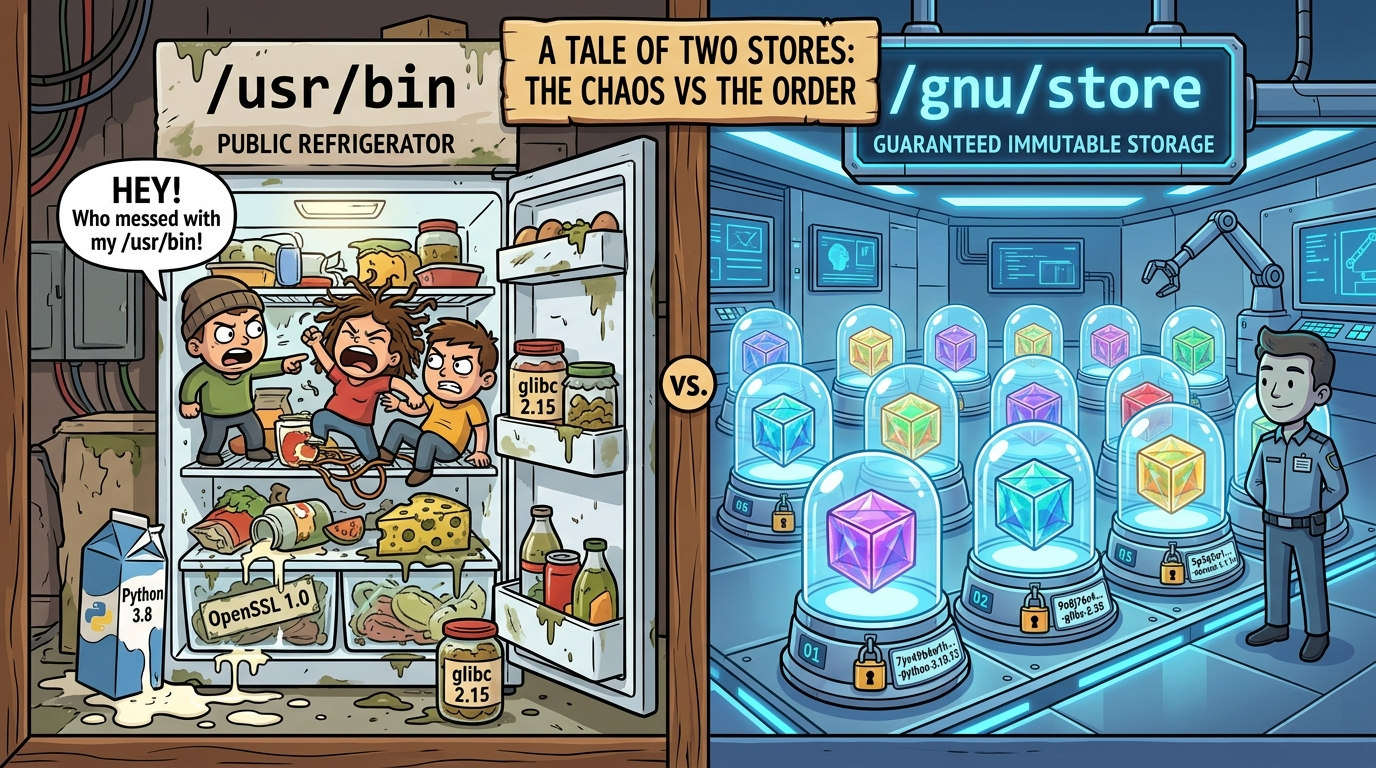
\includegraphics[width=0.92\textwidth]{images/store_vs_fridge.jpg}
\caption*{\textit{Figure 1.1: A Tale of Two Stores: The chaotic communal dorm fridge of \texttt{/usr/bin} versus the immutable crystal vault of \texttt{/gnu/store}.}}
\end{figure}

\section{Derivations: The Recipe Behind the Magic}

Before Guix builds anything, it generates a low-level recipe called a \textbf{Derivation} (stored as a \texttt{.drv} file in \texttt{/gnu/store}). 

A derivation is a completely serializable, language-agnostic description of an action to perform. You can think of it as an immutable build plan that specifies:
\begin{itemize}
  \item The inputs required (other store paths).
  \item The build environment (environment variables, architecture).
  \item The builder executable to invoke (often Guile or a shell script).
  \item The expected output paths in \texttt{/gnu/store}.
\end{itemize}

When you ask Guix to install or build a package, Guile evaluates your high-level Scheme code, translates it into a derivation graph (a Directed Acyclic Graph, or DAG), and hands it over to the background build daemon (\texttt{guix-daemon}).

\section{The Isolated Build Sandbox}

How does Guix guarantee that a build doesn't secretly depend on some random file sitting in \texttt{/tmp} or a global header file?

When the \texttt{guix-daemon} executes a derivation, it puts the build process inside an ultra-strict, isolated \textbf{chroot sandbox}:
\begin{enumerate}
  \item \textbf{No Network Access}: The builder has no internet connectivity during the build phase (unless it is a dedicated fixed-output download derivation with a verified cryptographic hash).
  \item \textbf{Clean Environment}: All host environment variables are stripped away. Only variables explicitly declared in the derivation exist.
  \item \textbf{Hermetic Filesystem}: The only files visible to the build process are the explicitly declared input store paths and an empty temporary build directory.
  \item \textbf{Time Travel to 1970}: The file timestamps inside the build directory are normalized to January 1, 1970, 00:00:01 UTC. This prevents build tools (like \texttt{zip} or \texttt{tar}) from baking non-deterministic timestamps into their binaries!
\end{enumerate}

\begin{footgunbox}[The Impure Build Assumption]
If you are used to building software on Ubuntu where your \texttt{Makefile} secretly relies on \texttt{/usr/include/some-header.h} that you installed five years ago and forgot about, Guix will immediately slap your hand and fail the build. In Guix, if an input is not explicitly declared in Scheme, it does not exist in the universe.
\end{footgunbox}

\section{Profiles and Generations: The Symlink Forest}

If everything is buried inside an unreadable hash path like:
\begin{center}
\storepath{/gnu/store/7yv4938r4wbz9p42x...-coreutils-9.1/bin/ls}
\end{center}
how on earth does a normal user run \texttt{ls} from their command line?

Guix solves this through \textbf{Profiles} and \textbf{Generations}.

\begin{itemize}
  \item A \textbf{Profile} is simply a directory containing symlinks pointing into various store paths. It mimics a standard Unix hierarchy (\texttt{bin/}, \texttt{lib/}, \texttt{share/}).
  \item Your shell's \texttt{\$PATH} simply points to \texttt{\textasciitilde/.guix-profile/bin}.
  \item Whenever you install or remove software, Guix builds a new store item representing the merged union of all your installed packages. This new union becomes \textbf{Generation $N+1$}.
  \item Guix updates the symlink \texttt{\textasciitilde/.guix-profile} to point to Generation $N+1$ using an \textbf{atomic rename} system call.
\end{itemize}

\begin{center}
\small
\begin{tabular}{r c l}
\toprule
\textbf{Symlink Pointer} & & \textbf{Target Destination} \\
\midrule
\texttt{\textasciitilde/.guix-profile} & $\longrightarrow$ & \texttt{/var/guix/profiles/per-user/alice/guix-profile} \\
\texttt{guix-profile} & $\longrightarrow$ & \texttt{guix-profile-42-link} \\
\texttt{guix-profile-42-link} & $\longrightarrow$ & \texttt{/gnu/store/...-profile/bin/ls} \\
\texttt{guix-profile-41-link} & $\longrightarrow$ & \texttt{/gnu/store/...-profile/bin/ls} (Rollback target) \\
\bottomrule
\end{tabular}
\end{center}

Because switching generations is literally just changing a single symbolic link, \textbf{installing packages is instantaneous and atomic}. If your laptop battery dies in the middle of a 4-gigabyte installation, your running profile is completely untouched. You cannot get a corrupted, half-installed system.

And if you hate the new version? You simply flip the symlink back to the previous generation.

\section{Two Operating Modes: Foreign Distros and Guix System}

Before we jump into the command line, one foundational distinction must be highlighted. GNU Guix can be operated in two fundamentally different modes:

\begin{enumerate}
  \item \textbf{As a Package Manager on a ``Foreign'' Distribution}: You install Guix on top of an existing, traditional Linux distribution such as Debian, Ubuntu, Fedora, openSUSE, or Arch Linux. In this setup, Guix coexists harmoniously alongside your host system's native package manager (\texttt{apt}, \texttt{dnf}, \texttt{pacman}). The host OS continues to handle your kernel, hardware drivers, and system daemons, while Guix provides an unprivileged, isolated \texttt{/gnu/store} and per-user profiles. You get reproducible packages, atomic rollbacks, and multi-version library coexistence without altering the underlying OS.
  \item \textbf{As a Complete Operating System (Guix System)}: Guix can also replace your entire traditional distribution. In Guix System, everything---from the Linux kernel, bootloader, Shepherd init system, and background daemons to user accounts and desktop environments---is declared within a unified Scheme configuration file (\texttt{/etc/config.scm}).
\end{enumerate}

Throughout Part~I and Part~II of this book, we will primarily explore Guix through the lens of a package manager running on a foreign distribution. As you will see in Chapter~\ref{chap:cli-daily-life}, the familiar, non-declarative commands for installing software (\texttt{guix install}) are uniquely suited to foreign distributions---whereas on Guix System, declarative configuration takes center stage.

